%%%%%%%%%%%%%%%%%%%%%%%%%%%%%%%%%%%%%%%%%%%%%%%%%%%%%%%%%%%%%%%%%%%%%%%%
%                                                                      %
%     File: Thesis_Introduction.tex                                    %
%     Tex Master: Thesis.tex                                           %
%                                                                      %
%     Author: Rui Santiago                         			   %
%     Last modified : 2 Junho 2015                         		   %
%                                                                      %
%%%%%%%%%%%%%%%%%%%%%%%%%%%%%%%%%%%%%%%%%%%%%%%%%%%%%%%%%%%%%%%%%%%%%%%%

\chapter{Compilador básico}
\label{chapter:Compilador basico}

Existem duas abordagens possíveis para realizar o compilador: fazer uma compilação clássica, através da construção de árvores de sintaxe abstracta ({\it abstract syntax trees}), cada uma representando uma expressão, realizando a respectiva decomposição e gerando as várias instruções. 

Outra abordagem que é analisada neste capítulo é fugir à implementação de um compilador clássico e utilizar uma linguagem de orientação por objectos para representar os componentes de {\it hardware}, onde cada classe é um componente de {\it hardware}. 
O programador utiliza essas classes com o objectivo de configurar o Data Engine.

Os métodos das classes permitem que o programador utilize as várias funções dos componentes de {\it hardware}. O programador utiliza as classes para descrever acções de controlo ou estruturas de {\it hardware} que permitam realizar a tarefa em questão.

O objectivo é construir uma linguagem de muito baixo nível para depois com o passar do tempo ser possível subir o nível de abstracção. 


\section{Abordagem da construção das árvores de sintaxe abstracta}
\label{section:Abordagem da construcao das arvores de sintaxe abstracta}

Construindo árvores de sintaxe abstracta é possível descodificar as expressões em instruções e gerar o respectivo {\it assembly}. A árvore de sintaxe abstracta é usada para analisar gramaticalmente as expressões. 

\subsection{Soma simples}
\label{subsection:Soma simples}

Considerando a soma de dois registos:

\begin{lstlisting} 
       R5 = R1+R2;      
\end{lstlisting}  
    
A árvore de análise respectiva encontra-se na figura~\ref{fig:Arvore_de sintaxe abstracta_de_uma_soma}.
No momento da construção da árvore, a árvore é percorrida da esquerda para a direita. A descodificação é feita pela seguinte ordem:

\begin{itemize}
  \item Entrada em R1 e memorização da instrução RDW, que vai executar uma leitura;
  \item Entrada em +, memorizando a instrução ADD;
  \item Entrada em R2, que vai indicar qual o regsto que se vai somar ao conteúdo do registo A;
  \item Gravar o resultado em R5, memorizando a instrução WRW.
\end{itemize}
    
    \begin{figure}[!htb]
  \centering
  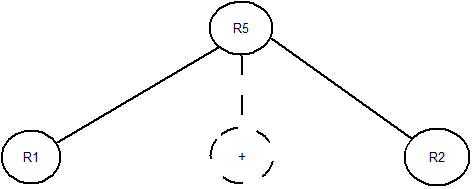
\includegraphics[height=45mm]{Figures/grafo1.png}
  \caption[Árvore lexical de uma soma.]{Árvore de sintaxe abstracta de uma soma.}  
  \label{fig:Arvore_de sintaxe abstracta_de_uma_soma}
\end{figure}
    
    O resultado é apenas gravado quando se termina a recursividade.
O respectivo código {\it assembly} é:

    RDW R1    

    ADD R2

    WRW R5
    
Esta abordagem é boa para compilar expressões para o controlador controlador, pois o controlador funciona como uma máquina convencional. No entanto, 
é uma abordagem menos boa para configurar e controlar o Data Engine.

\subsection{Ciclo {\it for}}
\label{subsection:Ciclo for}

Para a realização de um ciclo {\it for}, é necessário o uso do Data Engine. Considera-se o caso do ciclo {\it for} seguinte:

\begin{lstlisting}
    for (i=0;i<N;i++)    {
       MEM3[i] = MEM2[2i]+MEM2[2i+1];      }
\end{lstlisting}

Para o uso de ciclos {\it for}, não é necessário fazer a decomposição das expressões em instruções {\it assembly} usando compilação clássica, pois o Data Engine funciona de maneira diferente do controlador. No Data Engine usa-se instruções {\it assembly} apenas para sua configuração,
enquanto que no controlador cada expressão é descodificada para um equivalente em {\it assembly} para a execução. 
Conclui-se assim que para o Data Engine as árvores de sintaxe abstractas não são muito úteis.

\clearpage

\begin{figure}[!htb]
  \centering
  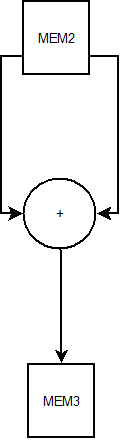
\includegraphics[height=90mm]{Figures/grafo2.png}
  \caption[Árvore lexical de uma soma]{Árvore lexical de uma soma dentro de um ciclo for}  
  \label{fig:Arvore_lexical_de_uma_soma_no_ciclo_for}
\end{figure}

Para o uso do Data Engine, é necessário usar um grafo em vez de uma árvore de sintaxe abstracta. Para um exemplo dado acima, construiu-se o grafo mostrado na figura~\ref{fig:Arvore_lexical_de_uma_soma_no_ciclo_for}. O compilador teria de identificar este grafo e depois controlar a execução do Data Engine. 

O código {\it assembly} que deveria ser produzido é dado a seguir:

\begin{lstlisting}
#clear conf_reg
	wrw CLEAR_CONFIG_ADDR
#configure mem2 for reading vectors x1 and x2
	ldi 0
	wrc MEM2A_CONFIG_ADDR,MEM_CONF_START_OFFSET
	ldi 1
	wrc MEM2B_CONFIG_ADDR,MEM_CONF_START_OFFSET
	ldi 1
	wrc MEM2A_CONFIG_ADDR,MEM_CONF_DUTY_OFFSET
	wrc MEM2B_CONFIG_ADDR,MEM_CONF_DUTY_OFFSET
	wrc MEM2A_CONFIG_ADDR,MEM_CONF_PER_OFFSET
	wrc MEM2B_CONFIG_ADDR,MEM_CONF_PER_OFFSET
	ldi 2
	wrc MEM2A_CONFIG_ADDR,MEM_CONF_INCR_OFFSET
	wrc MEM2B_CONFIG_ADDR,MEM_CONF_INCR_OFFSET
	ldi N
	wrc MEM2A_CONFIG_ADDR,MEM_CONF_ITER_OFFSET
	wrc MEM2B_CONFIG_ADDR,MEM_CONF_ITER_OFFSET
#configure mem3 for writing result
	ldi salu0
	wrc MEM3A_CONFIG_ADDR,MEM_CONF_SELA_OFFSET
	ldi 0
	wrc MEM3A_CONFIG_ADDR,MEM_CONF_START_OFFSET
	ldi 1
	wrc MEM3A_CONFIG_ADDR,MEM_CONF_DUTY_OFFSET
	wrc MEM3A_CONFIG_ADDR,MEM_CONF_PER_OFFSET
	wrc MEM3A_CONFIG_ADDR,MEM_CONF_INCR_OFFSET
	ldi 6
	wrc MEM3A_CONFIG_ADDR,MEM_CONF_DELAY_OFFSET
	ldi N
	wrc MEM3A_CONFIG_ADDR,MEM_CONF_ITER_OFFSET
#configure alu0 for adding x1 and x2
	ldi ALU_ADD
	wrc ALU0_CONFIG_ADDR,ALU_CONF_FNS_OFFSET
	ldi smul1
	wrc ALU0_CONFIG_ADDR,ALU_CONF_SELA_OFFSET
	ldi salu0
	wrc ALU0_CONFIG_ADDR,ALU_CONF_SELB_OFFSET
	ldi 1
#init engine
	ldi 0xfffd
	ldih 1
	wrw ENG_CTRL_REG
	wrw ENG_CTRL_REG
#run engine
	ldi 0xc002 
	ldih 1 
	wrw ENG_CTRL_REG
#wait for completion to display results
waitres	ldi 256
	and ENG_STATUS_REG
	beqi waitres
	nop
	nop
#branch to boot ROM
	ldi 0
	beqi 0
	nop
	nop
\end{lstlisting}

O número de iterações é definido por N, que é necessário indicar nos parâmetros \linebreak MEM{\_}CONF{\_}ITER{\_}OFFSET de cada memória usada. Visto que o i inicial é zero por pré-definição no compilador desenvolvido, 
os parâmetros MEM{\_}CONF{\_}INCR{\_}OFFSET e MEM{\_}CONF{\_}START{\_}OFFSET são usados para calcular os endereços na memória X da seguinte forma:

MEMx[INCR{\_}OFFSET*i+START{\_}OFFSET]

O gerador de endereços usado entre os dois disponíveis em cada memória é indicado pelo programador. Numa primeira abordagem, o período de cada iteração será também definido pelo programador. No futuro poderão usar-se mecanismos para automatizar o cálculo do período.

Os valores usados para inicializar e correr o Data Engine serão calculados internamente pelo compilador, recebendo instruções mais simples do utilizador. 

No ciclo {\it waitres} é usada uma máscara consoante a memória que se quer monitorizar. Quando uma memória acaba de ser lida ou escrita, é indicado no ENG{\_}STATUS{\_}REG que a memória terminou a sua execução.



\section{Utilização de uma linguagem orientada a objectos}
\label{section:Utilizacao de uma linguagem orientada a objectos}


A outra abordagem é através do uso de várias classes que representem os componentes do {\it Data Engine}. Utilizando esta abordagem, o programador escreve um programa com as classes disponíveis, descrevendo várias configurações do Data Engine.
Para as instruções do controlador, é usada uma linguagem interpretada. O UML das classes usadas no Data Engine é dado na figura~\ref{fig:tese_UML}.

%\begin{figure}[!htb]
 % \centering
 % 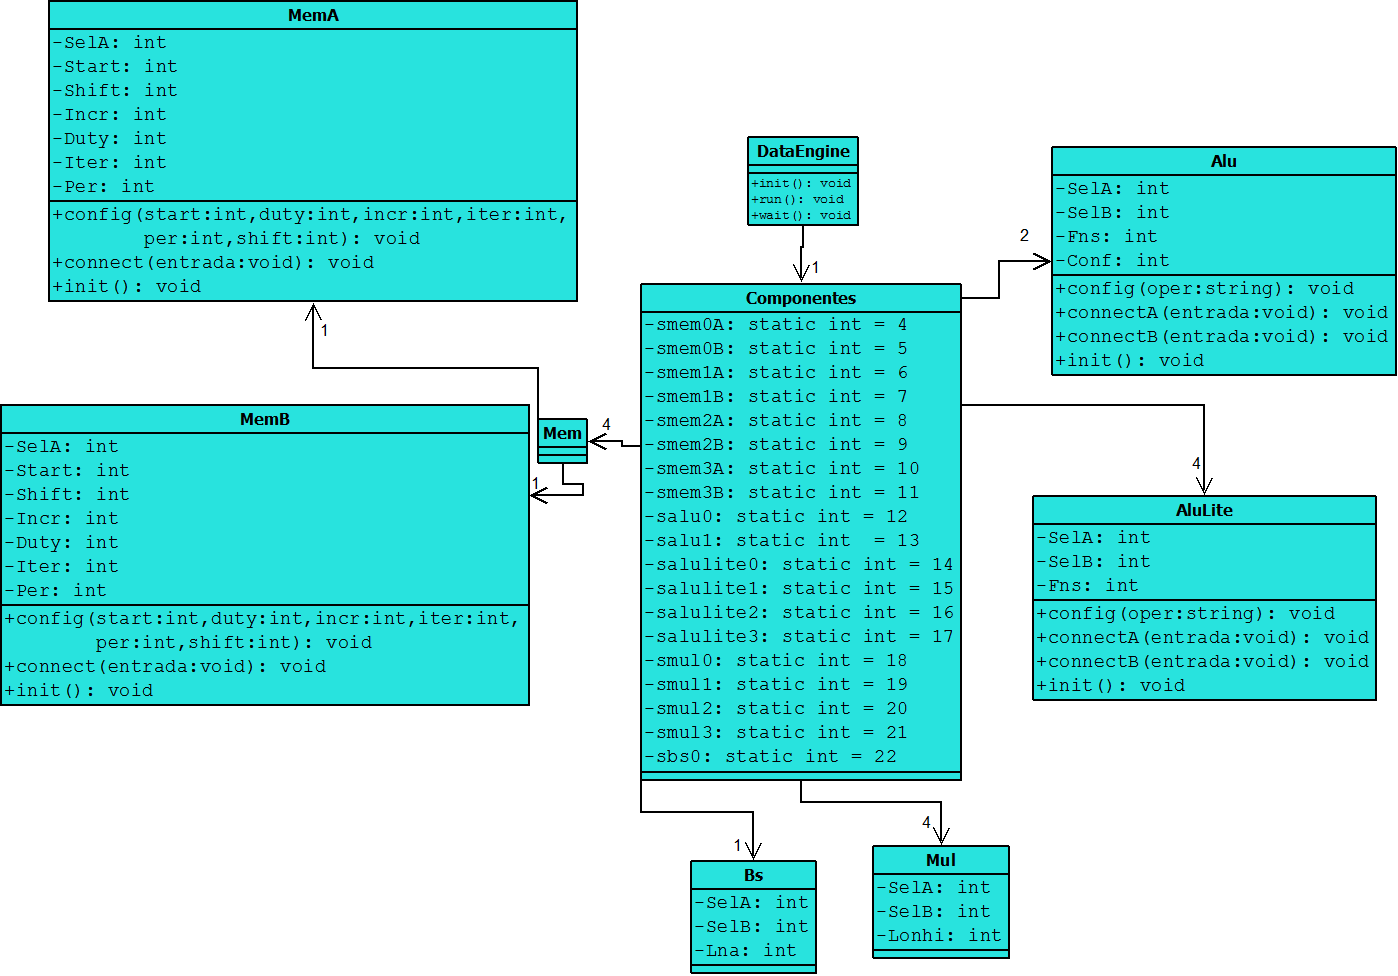
\includegraphics[height=175mm, angle=270, width=155mm]{Figures/tese_UML.png}
 % \caption[UML do Data Engine.]{UML do Data Engine.}  
%  \label{fig:tese_UML}
%\end{figure}

A compilação do código será feita pelo script automaticamente. Cada classe construirá o seu respectivo {\it Assembly}.

A nível do {\it Data Engine}, as ligações serão feitas directamente nas classes, que usando métodos do {\it Data Engine}, geram o próprio {\it Assembly}. 


%Para correr a instrução \begin{lstlisting} 
  %     R5 = R1+R2;      
%\end{lstlisting} é apenas necessário fazer

%R5=R1+R2





Considerando o exemplo da soma vectorial da secção anterior, o respectivo pseudo-código na linguagem Versat é:

\begin{lstlisting}

mem2A.config(0, 1, 2, N, 1, 0); // inicializar a memoria 2A
mem2B.config(1, 1, 2, N, 1, 0); // inicializar a memoria 2B
mem3A.config(0, 1, 6, N, 1, 0); // inicializar a memoria 3A

alu0.config("ADD"); // inicializar a alu

alu0.connectA(mem2A); // conectar a entrada A da alu a mem2A
alu0.connectB(mem2B); // conectar a entrada B da alu a mem2B

mem3A.connect(alu0); // conectar a memoria 3A a saida da ALU

mem2A.init(); // inicializar a memoria 2A
mem2B.init(); // inicializar a memoria 2B
mem3A.init(); // inicializar a memoria 3A
alu0.init(); // inicializar a alu0

mem3A.wait(); // marcar esta memoria para que se espere por ela


engine.init();
engine.run();
engine.wait();


\end{lstlisting}

Nos métodos de configuração das memórias, é passado o início, o
período, o {\it duty}, o incremento, o {\it delay} e o número de
iterações. De início decidiu-se passar também o {\it delay} mas
poderão vir a ser experimentadas formas de o compilador calcular o
{\it delay}.  A ALU precisa apenas de saber qual a operação que vai
realizar.

As conexões são feitas utilizando métodos do objecto destino. Existe
um método para cada conexão, um para a entrada A e outro para a
entrada B.

Como se pode ver, a descrição acima, usando um paradigma de
programação por objectos, consegue realizar a mesma função que o
código {\it assembly} dado para este exemplo. A diferença é que se
consegue uma descrição muito mais compacta e fácil de ler quando se
usa uma representação por objectos.

Poderia pensar-se em usar qualquer linguagem de programação orientada
para objectos para realizar descrições de configurações do Data Engine
e do seu controlo. Até se poderia usar uma linguagem de {\it
  scripting} como Python, a qual tem suporte para classes e
métodos. Estes programas quando executados gerariam o código assembly
ou o código máquina directamente. Esta abordagem evitaria de todo o
desenvolvimento de um {\em parser} para o compilador do Versat.

Contudo, uma parte importante do problema é compilar o código que é
corrido pelo controlador do Versat. Uma linguagem para esse fim seria
próxima de uma linguagem de programação convencional e teria de
incluir expressões condicionais ({\it if}) e ciclos de programa ({\it
  for, while, do while}, etc). Estas expressões são mais difíceis de
traduzir apenas chamando métodos de classes, e mesmo que se arranjasse
uma solução para tal, o código produzido não seria compacto e
elegante.


\begin{figure}[!htb]
  \centering
  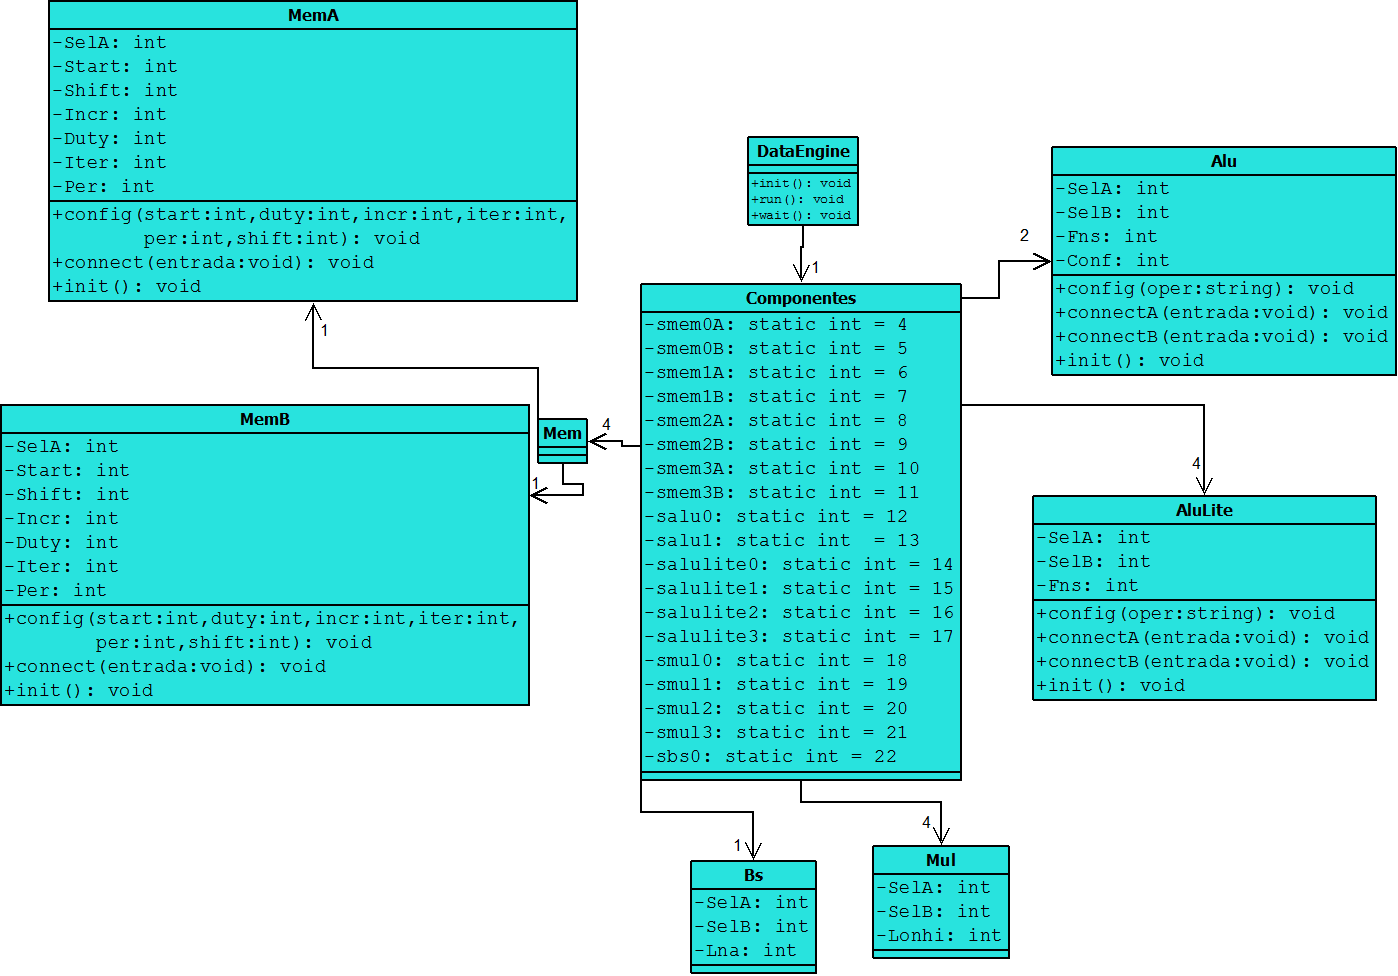
\includegraphics[height=105mm, angle=270, width=155mm]{Figures/tese_UML.png}
  \caption[UML do Data Engine.]{UML do Data Engine.}  
  \label{fig:tese_UML}
\end{figure}

\cleardoublepage
